\section{Supplementary pooling, metrics, and uncertainty}
\label{sec:supplement}
The supplementary \meanmodel{} uses training seed 44, the same five development folds, observed-history protocol, future-state objective, and forecast feature groups as \fullmodel{}, replacing spatial attention with mean pooling. Metrics are calculated separately from each fold model's predictions and then equally averaged. The per-fold results in Tables~\ref{tab:foldresults} and~\ref{tab:foldresults_forecast} retain the fitted-model estimates underlying the reported mean and sample standard deviation.
\begin{table*}[t]
\centering
\small
\caption{Supplementary spatial pooling comparison: mean $\pm$ sample fold SD of seed44 metrics. Each of the five fold models is evaluated separately; no probabilities are averaged. ForecastMean and ForecastAttention share forecast readout and future-state supervision.}
\label{tab:pooling}
\begin{tabular}{llrrr}
\toprule
Model & Landmark & AUROC & AP & F1 \\
\midrule
ForecastMean & T0 & 0.7317 $\pm$ 0.0094 & 0.5812 $\pm$ 0.0088 & 0.5446 $\pm$ 0.0406 \\
ForecastMean & T1 & 0.7367 $\pm$ 0.0100 & 0.5869 $\pm$ 0.0191 & 0.5523 $\pm$ 0.0312 \\
ForecastMean & T2 & 0.7361 $\pm$ 0.0103 & 0.5856 $\pm$ 0.0189 & 0.5405 $\pm$ 0.0172 \\
ForecastMean & Macro & 0.7348 $\pm$ 0.0092 & 0.5845 $\pm$ 0.0145 & 0.5458 $\pm$ 0.0225 \\
ForecastAttention & T0 & 0.7294 $\pm$ 0.0171 & 0.5924 $\pm$ 0.0124 & 0.5334 $\pm$ 0.0350 \\
ForecastAttention & T1 & 0.7381 $\pm$ 0.0161 & 0.6012 $\pm$ 0.0156 & 0.5563 $\pm$ 0.0330 \\
ForecastAttention & T2 & 0.7421 $\pm$ 0.0167 & 0.6033 $\pm$ 0.0191 & 0.5510 $\pm$ 0.0427 \\
ForecastAttention & Macro & 0.7365 $\pm$ 0.0159 & 0.5990 $\pm$ 0.0151 & 0.5469 $\pm$ 0.0334 \\
\bottomrule
\end{tabular}
\end{table*}

\begin{table*}[t]
\centering
\small
\caption{Individual seed44 fold-model results for direct readouts. Each fold model is evaluated separately on the same 175 patients (56 positive), without averaging probabilities. Macro averages the three landmark metrics. The folds are overlapping training partitions, not independent test cohorts.}
\label{tab:foldresults}
\begin{tabular}{llrrrr}
\toprule
Model & Fold & Landmark & AUROC & AP & F1 \\
\midrule
NoJEPA & 1 & T0 & 0.7131 & 0.5718 & 0.5254 \\
NoJEPA & 1 & T1 & 0.7165 & 0.5952 & 0.5469 \\
NoJEPA & 1 & T2 & 0.7150 & 0.5872 & 0.5299 \\
NoJEPA & 1 & Macro & 0.7149 & 0.5848 & 0.5341 \\
NoJEPA & 2 & T0 & 0.7339 & 0.6042 & 0.5758 \\
NoJEPA & 2 & T1 & 0.7332 & 0.5959 & 0.6061 \\
NoJEPA & 2 & T2 & 0.7342 & 0.5986 & 0.6000 \\
NoJEPA & 2 & Macro & 0.7338 & 0.5996 & 0.5939 \\
NoJEPA & 3 & T0 & 0.7090 & 0.5267 & 0.5354 \\
NoJEPA & 3 & T1 & 0.7110 & 0.5506 & 0.5246 \\
NoJEPA & 3 & T2 & 0.7149 & 0.5588 & 0.5238 \\
NoJEPA & 3 & Macro & 0.7116 & 0.5453 & 0.5279 \\
NoJEPA & 4 & T0 & 0.7156 & 0.5811 & 0.4957 \\
NoJEPA & 4 & T1 & 0.7137 & 0.5809 & 0.4959 \\
NoJEPA & 4 & T2 & 0.7147 & 0.5817 & 0.4918 \\
NoJEPA & 4 & Macro & 0.7147 & 0.5812 & 0.4945 \\
NoJEPA & 5 & T0 & 0.7330 & 0.5906 & 0.5882 \\
NoJEPA & 5 & T1 & 0.7350 & 0.5851 & 0.5556 \\
NoJEPA & 5 & T2 & 0.7362 & 0.5795 & 0.5600 \\
NoJEPA & 5 & Macro & 0.7347 & 0.5851 & 0.5679 \\
DirectReadout & 1 & T0 & 0.7305 & 0.5843 & 0.5426 \\
DirectReadout & 1 & T1 & 0.7291 & 0.5796 & 0.5672 \\
DirectReadout & 1 & T2 & 0.7291 & 0.5790 & 0.5857 \\
DirectReadout & 1 & Macro & 0.7296 & 0.5810 & 0.5652 \\
DirectReadout & 2 & T0 & 0.7372 & 0.6104 & 0.5424 \\
DirectReadout & 2 & T1 & 0.7374 & 0.6141 & 0.5500 \\
DirectReadout & 2 & T2 & 0.7350 & 0.6141 & 0.6087 \\
DirectReadout & 2 & Macro & 0.7365 & 0.6129 & 0.5670 \\
DirectReadout & 3 & T0 & 0.7150 & 0.5940 & 0.5041 \\
DirectReadout & 3 & T1 & 0.7179 & 0.6003 & 0.5203 \\
DirectReadout & 3 & T2 & 0.7183 & 0.6019 & 0.5197 \\
DirectReadout & 3 & Macro & 0.7171 & 0.5987 & 0.5147 \\
DirectReadout & 4 & T0 & 0.7203 & 0.5554 & 0.5455 \\
DirectReadout & 4 & T1 & 0.7213 & 0.5552 & 0.5455 \\
DirectReadout & 4 & T2 & 0.7201 & 0.5586 & 0.5620 \\
DirectReadout & 4 & Macro & 0.7206 & 0.5564 & 0.5510 \\
DirectReadout & 5 & T0 & 0.7489 & 0.5832 & 0.5891 \\
DirectReadout & 5 & T1 & 0.7473 & 0.5964 & 0.5593 \\
DirectReadout & 5 & T2 & 0.7468 & 0.6062 & 0.5667 \\
DirectReadout & 5 & Macro & 0.7477 & 0.5953 & 0.5717 \\
\bottomrule
\end{tabular}
\end{table*}

\begin{table*}[t]
\centering
\small
\caption{Individual seed44 fold-model results for forecast readouts. Evaluation and aggregation match Table~\ref{tab:foldresults}; these individual fold metrics generate the mean and sample SD in the main tables.}
\label{tab:foldresults_forecast}
\begin{tabular}{llrrrr}
\toprule
Model & Fold & Landmark & AUROC & AP & F1 \\
\midrule
ForecastAttention & 1 & T0 & 0.7449 & 0.6015 & 0.5802 \\
ForecastAttention & 1 & T1 & 0.7410 & 0.6033 & 0.6056 \\
ForecastAttention & 1 & T2 & 0.7407 & 0.5973 & 0.6074 \\
ForecastAttention & 1 & Macro & 0.7422 & 0.6007 & 0.5977 \\
ForecastAttention & 2 & T0 & 0.7423 & 0.6024 & 0.5591 \\
ForecastAttention & 2 & T1 & 0.7584 & 0.6218 & 0.5514 \\
ForecastAttention & 2 & T2 & 0.7688 & 0.6311 & 0.5288 \\
ForecastAttention & 2 & Macro & 0.7565 & 0.6185 & 0.5464 \\
ForecastAttention & 3 & T0 & 0.7368 & 0.5952 & 0.5047 \\
ForecastAttention & 3 & T1 & 0.7471 & 0.6010 & 0.5179 \\
ForecastAttention & 3 & T2 & 0.7446 & 0.6048 & 0.5470 \\
ForecastAttention & 3 & Macro & 0.7428 & 0.6003 & 0.5232 \\
ForecastAttention & 4 & T0 & 0.7176 & 0.5909 & 0.5000 \\
ForecastAttention & 4 & T1 & 0.7237 & 0.6021 & 0.5389 \\
ForecastAttention & 4 & T2 & 0.7311 & 0.6054 & 0.4961 \\
ForecastAttention & 4 & Macro & 0.7241 & 0.5995 & 0.5117 \\
ForecastAttention & 5 & T0 & 0.7056 & 0.5719 & 0.5231 \\
ForecastAttention & 5 & T1 & 0.7200 & 0.5780 & 0.5676 \\
ForecastAttention & 5 & T2 & 0.7254 & 0.5780 & 0.5755 \\
ForecastAttention & 5 & Macro & 0.7170 & 0.5759 & 0.5554 \\
ForecastMean & 1 & T0 & 0.7369 & 0.5746 & 0.5600 \\
ForecastMean & 1 & T1 & 0.7469 & 0.5831 & 0.5882 \\
ForecastMean & 1 & T2 & 0.7482 & 0.5963 & 0.5556 \\
ForecastMean & 1 & Macro & 0.7440 & 0.5846 & 0.5679 \\
ForecastMean & 2 & T0 & 0.7458 & 0.5702 & 0.6015 \\
ForecastMean & 2 & T1 & 0.7458 & 0.5670 & 0.5487 \\
ForecastMean & 2 & T2 & 0.7458 & 0.5666 & 0.5192 \\
ForecastMean & 2 & Macro & 0.7458 & 0.5679 & 0.5565 \\
ForecastMean & 3 & T0 & 0.7263 & 0.5922 & 0.4906 \\
ForecastMean & 3 & T1 & 0.7248 & 0.6119 & 0.5045 \\
ForecastMean & 3 & T2 & 0.7321 & 0.6038 & 0.5299 \\
ForecastMean & 3 & Macro & 0.7277 & 0.6026 & 0.5083 \\
ForecastMean & 4 & T0 & 0.7251 & 0.5856 & 0.5399 \\
ForecastMean & 4 & T1 & 0.7285 & 0.6009 & 0.5506 \\
ForecastMean & 4 & T2 & 0.7290 & 0.5975 & 0.5600 \\
ForecastMean & 4 & Macro & 0.7275 & 0.5946 & 0.5501 \\
ForecastMean & 5 & T0 & 0.7242 & 0.5833 & 0.5312 \\
ForecastMean & 5 & T1 & 0.7377 & 0.5716 & 0.5693 \\
ForecastMean & 5 & T2 & 0.7252 & 0.5636 & 0.5378 \\
ForecastMean & 5 & Macro & 0.7290 & 0.5728 & 0.5461 \\
\bottomrule
\end{tabular}
\end{table*}

\begin{table*}[t]
\centering
\footnotesize
\setlength{\tabcolsep}{5pt}
\caption{All 14 macro metrics for the principal variants: point estimate [95\% patient-bootstrap percentile interval]. Metrics are computed separately for each seed44 fold model, averaged over T0--T2 within fold, then equally averaged over five folds. Probabilities are not averaged. Threshold-dependent metrics use 0.5. Identical patient resamples preserve pairing across models and landmarks. Entries are marginal model intervals; paired differences are reported separately. Intervals condition on the fitted fold models and exclude retraining and retrospective selection uncertainty. Downward arrows identify metrics for which lower is better.}
\label{tab:extended_macro}
\begin{tabular}{lccc}
\toprule
Metric & NoJEPA & DirectReadout & ForecastAttention \\
\midrule
AUROC & 0.7219 [0.6422, 0.7931] & 0.7303 [0.6514, 0.7999] & 0.7365 [0.6602, 0.8040] \\
AP & 0.5792 [0.4646, 0.6913] & 0.5888 [0.4769, 0.7000] & 0.5990 [0.4891, 0.7082] \\
F1 & 0.5437 [0.4433, 0.6293] & 0.5539 [0.4575, 0.6374] & 0.5469 [0.4551, 0.6199] \\
Accuracy & 0.6743 [0.6137, 0.7349] & 0.6731 [0.6130, 0.7299] & 0.6290 [0.5752, 0.6777] \\
Sensitivity & 0.6095 [0.4930, 0.7183] & 0.6357 [0.5321, 0.7436] & 0.7036 [0.6125, 0.7877] \\
Specificity & 0.7048 [0.6319, 0.7728] & 0.6908 [0.6162, 0.7593] & 0.5938 [0.5291, 0.6573] \\
PPV & 0.4921 [0.3813, 0.5991] & 0.4938 [0.3874, 0.5960] & 0.4643 [0.3679, 0.5562] \\
NPV & 0.7943 [0.7164, 0.8632] & 0.8023 [0.7229, 0.8713] & 0.8269 [0.7559, 0.8879] \\
Balanced accuracy & 0.6571 [0.5887, 0.7234] & 0.6632 [0.5960, 0.7269] & 0.6487 [0.5913, 0.7004] \\
MCC & 0.3000 [0.1683, 0.4237] & 0.3109 [0.1828, 0.4305] & 0.2931 [0.1808, 0.3874] \\
Youden index & 0.3143 [0.1774, 0.4468] & 0.3265 [0.1920, 0.4538] & 0.2974 [0.1826, 0.4009] \\
NLL $\downarrow$ & 0.5974 [0.5344, 0.6665] & 0.5995 [0.5387, 0.6660] & 0.6149 [0.5778, 0.6548] \\
Brier score $\downarrow$ & 0.2069 [0.1795, 0.2358] & 0.2073 [0.1812, 0.2352] & 0.2147 [0.1979, 0.2327] \\
ECE $\downarrow$ & 0.1310 [0.1104, 0.1963] & 0.1377 [0.1142, 0.2002] & 0.1622 [0.1260, 0.2265] \\
\bottomrule
\end{tabular}
\end{table*}

\begin{table*}[t]
\centering
\small
\caption{Threshold sensitivity analysis: seed44 five-fold metric means. Each fold model uses its own landmark-specific validation Youden threshold on the holdout scores from the same model. Validation also informed best-checkpoint selection; this is sensitivity analysis, not nested calibration. No test labels choose thresholds.}
\label{tab:extended_threshold}
\begin{tabular}{llrrrr}
\toprule
Model & Policy & F1 & Sens. & Spec. & MCC \\
\midrule
NoJEPA & 0.5 & 0.544 & 0.610 & 0.705 & 0.300 \\
NoJEPA & Fold validation Youden & 0.551 & 0.645 & 0.675 & 0.303 \\
\midrule
DirectReadout & 0.5 & 0.554 & 0.636 & 0.691 & 0.311 \\
DirectReadout & Fold validation Youden & 0.537 & 0.581 & 0.734 & 0.310 \\
\midrule
ForecastAttention & 0.5 & 0.547 & 0.704 & 0.594 & 0.293 \\
ForecastAttention & Fold validation Youden & 0.541 & 0.644 & 0.656 & 0.288 \\
\bottomrule
\end{tabular}
\end{table*}


\subsection{Paired significance checks}
Table~\ref{tab:bootstrap} reports the nine principal Macro comparisons, with unadjusted 95\% paired patient-bootstrap intervals, raw two-sided approximate bootstrap $p$ values, within-family Holm adjustment, and all-90 Holm adjustment. The secondary family comprises 81 tests in Tables~\ref{tab:significance_landmarks}--\ref{tab:significance_longitudinal}. Every patient draw is shared across all five fixed fold models, variants, and landmarks. Metrics are recomputed separately for each fold before averaging, so the independent patient count remains 175. A significance marker refers to the stated Holm-adjusted family; ns denotes $p_{\mathrm{Holm}}\geq0.05$. The 2,000-resample percentile intervals are unadjusted and are not exact inversions of the 99,999-resample null-centered tests. All testing and reporting choices remain retrospective and exploratory.

\begin{table*}[t]
\centering
\small
\caption{Exploratory landmark comparisons. All metrics use approximate, null-centered paired patient-bootstrap tests (99,999 shared draws across folds, models, and landmarks). All $p$ values are two-sided. $p_{\mathrm{Holm}}$ adjusts jointly over the 81 secondary tests in Tables~\ref{tab:significance_landmarks}--\ref{tab:significance_longitudinal}. Direct and Attention abbreviate DirectReadout and ForecastAttention. $^{*}p_{\mathrm{Holm}}<0.05$, $^{**}p_{\mathrm{Holm}}<0.01$, $^{***}p_{\mathrm{Holm}}<0.001$; ns, not significant after the stated correction. Intervals are unadjusted 95\% patient-bootstrap intervals (2,000 shared draws) and need not agree with adjusted test decisions. All analyses condition on the five fixed seed44 fold models; folds are not resampled and share one holdout.}
\label{tab:significance_landmarks}
\begin{tabular}{lllrrrc}
\toprule
Comparison & Landmark & Metric & Difference [95\% CI] & $p$ & $p_{\mathrm{Holm}}$ & Sig. \\
\midrule
Direct -- NoJEPA & T0 & AUROC & +0.0095 [-0.0043, +0.0234] & 0.1953 & 1.0000 & ns \\
Direct -- NoJEPA & T0 & AP & +0.0106 [-0.0125, +0.0301] & 0.3397 & 1.0000 & ns \\
Direct -- NoJEPA & T0 & F1 & +0.0006 [-0.0275, +0.0282] & 0.9656 & 1.0000 & ns \\
Direct -- NoJEPA & T1 & AUROC & +0.0087 [-0.0050, +0.0224] & 0.2221 & 1.0000 & ns \\
Direct -- NoJEPA & T1 & AP & +0.0076 [-0.0156, +0.0311] & 0.5254 & 1.0000 & ns \\
Direct -- NoJEPA & T1 & F1 & +0.0027 [-0.0212, +0.0258] & 0.8279 & 1.0000 & ns \\
Direct -- NoJEPA & T2 & AUROC & +0.0069 [-0.0061, +0.0198] & 0.3084 & 1.0000 & ns \\
Direct -- NoJEPA & T2 & AP & +0.0108 [-0.0104, +0.0314] & 0.3172 & 1.0000 & ns \\
Direct -- NoJEPA & T2 & F1 & +0.0274 [+0.0029, +0.0542] & 0.0309 & 1.0000 & ns \\
Attention -- NoJEPA & T0 & AUROC & +0.0085 [-0.0171, +0.0346] & 0.5060 & 1.0000 & ns \\
Attention -- NoJEPA & T0 & AP & +0.0175 [-0.0245, +0.0633] & 0.4277 & 1.0000 & ns \\
Attention -- NoJEPA & T0 & F1 & -0.0107 [-0.0504, +0.0274] & 0.5972 & 1.0000 & ns \\
Attention -- NoJEPA & T1 & AUROC & +0.0162 [-0.0062, +0.0400] & 0.1564 & 1.0000 & ns \\
Attention -- NoJEPA & T1 & AP & +0.0197 [-0.0174, +0.0632] & 0.3221 & 1.0000 & ns \\
Attention -- NoJEPA & T1 & F1 & +0.0105 [-0.0329, +0.0546] & 0.6422 & 1.0000 & ns \\
Attention -- NoJEPA & T2 & AUROC & +0.0191 [-0.0017, +0.0405] & 0.0710 & 1.0000 & ns \\
Attention -- NoJEPA & T2 & AP & +0.0222 [-0.0114, +0.0614] & 0.2241 & 1.0000 & ns \\
Attention -- NoJEPA & T2 & F1 & +0.0099 [-0.0268, +0.0454] & 0.5894 & 1.0000 & ns \\
Attention -- Direct & T0 & AUROC & -0.0010 [-0.0246, +0.0240] & 0.9373 & 1.0000 & ns \\
Attention -- Direct & T0 & AP & +0.0069 [-0.0288, +0.0492] & 0.7232 & 1.0000 & ns \\
Attention -- Direct & T0 & F1 & -0.0113 [-0.0510, +0.0282] & 0.5821 & 1.0000 & ns \\
Attention -- Direct & T1 & AUROC & +0.0074 [-0.0132, +0.0292] & 0.4835 & 1.0000 & ns \\
Attention -- Direct & T1 & AP & +0.0121 [-0.0256, +0.0557] & 0.5427 & 1.0000 & ns \\
Attention -- Direct & T1 & F1 & +0.0078 [-0.0305, +0.0480] & 0.6869 & 1.0000 & ns \\
Attention -- Direct & T2 & AUROC & +0.0122 [-0.0064, +0.0313] & 0.2146 & 1.0000 & ns \\
Attention -- Direct & T2 & AP & +0.0113 [-0.0217, +0.0506] & 0.5265 & 1.0000 & ns \\
Attention -- Direct & T2 & F1 & -0.0176 [-0.0497, +0.0135] & 0.2732 & 1.0000 & ns \\
\bottomrule
\end{tabular}
\end{table*}

\begin{table*}[t]
\centering
\small
\caption{Exploratory Macro operating and probability-quality comparisons. Differences are first-named minus second-named model; negative Brier, NLL, or ECE differences favor the first model. All metrics use approximate, null-centered paired patient-bootstrap tests (99,999 shared draws across folds, models, and landmarks). All $p$ values are two-sided. $p_{\mathrm{Holm}}$ adjusts jointly over the 81 secondary tests in Tables~\ref{tab:significance_landmarks}--\ref{tab:significance_longitudinal}. Direct and Attention abbreviate DirectReadout and ForecastAttention. $^{*}p_{\mathrm{Holm}}<0.05$, $^{**}p_{\mathrm{Holm}}<0.01$, $^{***}p_{\mathrm{Holm}}<0.001$; ns, not significant after the stated correction. Intervals are unadjusted 95\% patient-bootstrap intervals (2,000 shared draws) and need not agree with adjusted test decisions. All analyses condition on the five fixed seed44 fold models; folds are not resampled and share one holdout.}
\label{tab:significance_extended}
\begin{tabular}{llrrrc}
\toprule
Comparison & Metric & Difference [95\% CI] & $p$ & $p_{\mathrm{Holm}}$ & Sig. \\
\midrule
Direct -- NoJEPA & Accuracy & -0.0011 [-0.0187, +0.0152] & 0.9142 & 1.0000 & ns \\
Direct -- NoJEPA & Sensitivity & +0.0262 [-0.0011, +0.0560] & 0.0820 & 1.0000 & ns \\
Direct -- NoJEPA & Specificity & -0.0140 [-0.0361, +0.0062] & 0.1997 & 1.0000 & ns \\
Direct -- NoJEPA & PPV & +0.0017 [-0.0202, +0.0232] & 0.8776 & 1.0000 & ns \\
Direct -- NoJEPA & NPV & +0.0080 [-0.0054, +0.0216] & 0.2505 & 1.0000 & ns \\
Direct -- NoJEPA & Balanced accuracy & +0.0061 [-0.0119, +0.0241] & 0.5082 & 1.0000 & ns \\
Direct -- NoJEPA & MCC & +0.0109 [-0.0233, +0.0453] & 0.5391 & 1.0000 & ns \\
Direct -- NoJEPA & Youden index & +0.0122 [-0.0237, +0.0482] & 0.5082 & 1.0000 & ns \\
Direct -- NoJEPA & Brier & +0.0003 [-0.0050, +0.0057] & 0.9099 & 1.0000 & ns \\
Direct -- NoJEPA & NLL & +0.0021 [-0.0113, +0.0156] & 0.7649 & 1.0000 & ns \\
Direct -- NoJEPA & ECE & +0.0067 [-0.0191, +0.0242] & 0.5498 & 1.0000 & ns \\
Attention -- NoJEPA & Accuracy & -0.0453 [-0.0781, -0.0149] & 0.0044 & 0.3352 & ns \\
Attention -- NoJEPA & Sensitivity & +0.0940 [+0.0483, +0.1422] & 0.0004 & 0.0300 & * \\
Attention -- NoJEPA & Specificity & -0.1109 [-0.1459, -0.0779] & $<0.0001$ & 0.0008 & *** \\
Attention -- NoJEPA & PPV & -0.0278 [-0.0652, +0.0033] & 0.1083 & 1.0000 & ns \\
Attention -- NoJEPA & NPV & +0.0326 [+0.0075, +0.0584] & 0.0149 & 1.0000 & ns \\
Attention -- NoJEPA & Balanced accuracy & -0.0084 [-0.0387, +0.0194] & 0.5721 & 1.0000 & ns \\
Attention -- NoJEPA & MCC & -0.0069 [-0.0648, +0.0463] & 0.8099 & 1.0000 & ns \\
Attention -- NoJEPA & Youden index & -0.0169 [-0.0774, +0.0387] & 0.5721 & 1.0000 & ns \\
Attention -- NoJEPA & Brier & +0.0078 [-0.0054, +0.0207] & 0.2409 & 1.0000 & ns \\
Attention -- NoJEPA & NLL & +0.0176 [-0.0152, +0.0490] & 0.2809 & 1.0000 & ns \\
Attention -- NoJEPA & ECE & +0.0312 [-0.0121, +0.0507] & 0.0906 & 1.0000 & ns \\
Attention -- Direct & Accuracy & -0.0442 [-0.0724, -0.0175] & 0.0014 & 0.1123 & ns \\
Attention -- Direct & Sensitivity & +0.0679 [+0.0262, +0.1103] & 0.0021 & 0.1586 & ns \\
Attention -- Direct & Specificity & -0.0969 [-0.1280, -0.0685] & $<0.0001$ & 0.0008 & *** \\
Attention -- Direct & PPV & -0.0295 [-0.0607, -0.0019] & 0.0519 & 1.0000 & ns \\
Attention -- Direct & NPV & +0.0246 [+0.0014, +0.0485] & 0.0390 & 1.0000 & ns \\
Attention -- Direct & Balanced accuracy & -0.0145 [-0.0419, +0.0104] & 0.2732 & 1.0000 & ns \\
Attention -- Direct & MCC & -0.0178 [-0.0695, +0.0300] & 0.4783 & 1.0000 & ns \\
Attention -- Direct & Youden index & -0.0291 [-0.0838, +0.0209] & 0.2732 & 1.0000 & ns \\
Attention -- Direct & Brier & +0.0075 [-0.0052, +0.0194] & 0.2189 & 1.0000 & ns \\
Attention -- Direct & NLL & +0.0155 [-0.0146, +0.0439] & 0.2952 & 1.0000 & ns \\
Attention -- Direct & ECE & +0.0245 [-0.0070, +0.0403] & 0.0685 & 1.0000 & ns \\
\bottomrule
\end{tabular}
\end{table*}

\begin{table*}[t]
\centering
\small
\caption{Exploratory pooling comparisons: ForecastAttention minus ForecastMean. All metrics use approximate, null-centered paired patient-bootstrap tests (99,999 shared draws across folds, models, and landmarks). All $p$ values are two-sided. $p_{\mathrm{Holm}}$ adjusts jointly over the 81 secondary tests in Tables~\ref{tab:significance_landmarks}--\ref{tab:significance_longitudinal}. Direct and Attention abbreviate DirectReadout and ForecastAttention. $^{*}p_{\mathrm{Holm}}<0.05$, $^{**}p_{\mathrm{Holm}}<0.01$, $^{***}p_{\mathrm{Holm}}<0.001$; ns, not significant after the stated correction. Intervals are unadjusted 95\% patient-bootstrap intervals (2,000 shared draws) and need not agree with adjusted test decisions. All analyses condition on the five fixed seed44 fold models; folds are not resampled and share one holdout.}
\label{tab:significance_pooling}
\begin{tabular}{llrrrc}
\toprule
Landmark & Metric & Difference [95\% CI] & $p$ & $p_{\mathrm{Holm}}$ & Sig. \\
\midrule
T0 & AUROC & -0.0022 [-0.0234, +0.0191] & 0.8273 & 1.0000 & ns \\
T0 & AP & +0.0112 [-0.0194, +0.0465] & 0.5022 & 1.0000 & ns \\
T0 & F1 & -0.0112 [-0.0516, +0.0289] & 0.5810 & 1.0000 & ns \\
T1 & AUROC & +0.0013 [-0.0174, +0.0203] & 0.8900 & 1.0000 & ns \\
T1 & AP & +0.0144 [-0.0154, +0.0469] & 0.3622 & 1.0000 & ns \\
T1 & F1 & +0.0040 [-0.0212, +0.0282] & 0.7540 & 1.0000 & ns \\
T2 & AUROC & +0.0060 [-0.0125, +0.0252] & 0.5291 & 1.0000 & ns \\
T2 & AP & +0.0178 [-0.0103, +0.0470] & 0.2229 & 1.0000 & ns \\
T2 & F1 & +0.0105 [-0.0220, +0.0450] & 0.5512 & 1.0000 & ns \\
Macro & AUROC & +0.0017 [-0.0169, +0.0207] & 0.8580 & 1.0000 & ns \\
Macro & AP & +0.0144 [-0.0145, +0.0453] & 0.3380 & 1.0000 & ns \\
Macro & F1 & +0.0011 [-0.0237, +0.0271] & 0.9351 & 1.0000 & ns \\
\bottomrule
\end{tabular}
\end{table*}

\begin{table*}[t]
\centering
\small
\caption{Exploratory paired T2 minus T0 comparisons. Shared patient-bootstrap draws retain dependence between folds and landmarks. All metrics use approximate, null-centered paired patient-bootstrap tests (99,999 shared draws across folds, models, and landmarks). All $p$ values are two-sided. $p_{\mathrm{Holm}}$ adjusts jointly over the 81 secondary tests in Tables~\ref{tab:significance_landmarks}--\ref{tab:significance_longitudinal}. Direct and Attention abbreviate DirectReadout and ForecastAttention. $^{*}p_{\mathrm{Holm}}<0.05$, $^{**}p_{\mathrm{Holm}}<0.01$, $^{***}p_{\mathrm{Holm}}<0.001$; ns, not significant after the stated correction. Intervals are unadjusted 95\% patient-bootstrap intervals (2,000 shared draws) and need not agree with adjusted test decisions. All analyses condition on the five fixed seed44 fold models; folds are not resampled and share one holdout.}
\label{tab:significance_longitudinal}
\begin{tabular}{llrrrc}
\toprule
Model & Metric & Difference [95\% CI] & $p$ & $p_{\mathrm{Holm}}$ & Sig. \\
\midrule
NoJEPA & AUROC & +0.0021 [-0.0027, +0.0073] & 0.4258 & 1.0000 & ns \\
NoJEPA & AP & +0.0063 [-0.0093, +0.0197] & 0.4193 & 1.0000 & ns \\
NoJEPA & F1 & -0.0030 [-0.0163, +0.0091] & 0.6396 & 1.0000 & ns \\
DirectReadout & AUROC & -0.0005 [-0.0086, +0.0081] & 0.9031 & 1.0000 & ns \\
DirectReadout & AP & +0.0065 [-0.0062, +0.0189] & 0.3131 & 1.0000 & ns \\
DirectReadout & F1 & +0.0238 [+0.0009, +0.0478] & 0.0443 & 1.0000 & ns \\
ForecastAttention & AUROC & +0.0127 [+0.0026, +0.0235] & 0.0189 & 1.0000 & ns \\
ForecastAttention & AP & +0.0110 [-0.0048, +0.0264] & 0.1848 & 1.0000 & ns \\
ForecastAttention & F1 & +0.0176 [-0.0051, +0.0424] & 0.1341 & 1.0000 & ns \\
\bottomrule
\end{tabular}
\end{table*}


\begin{figure*}[t]
\centering
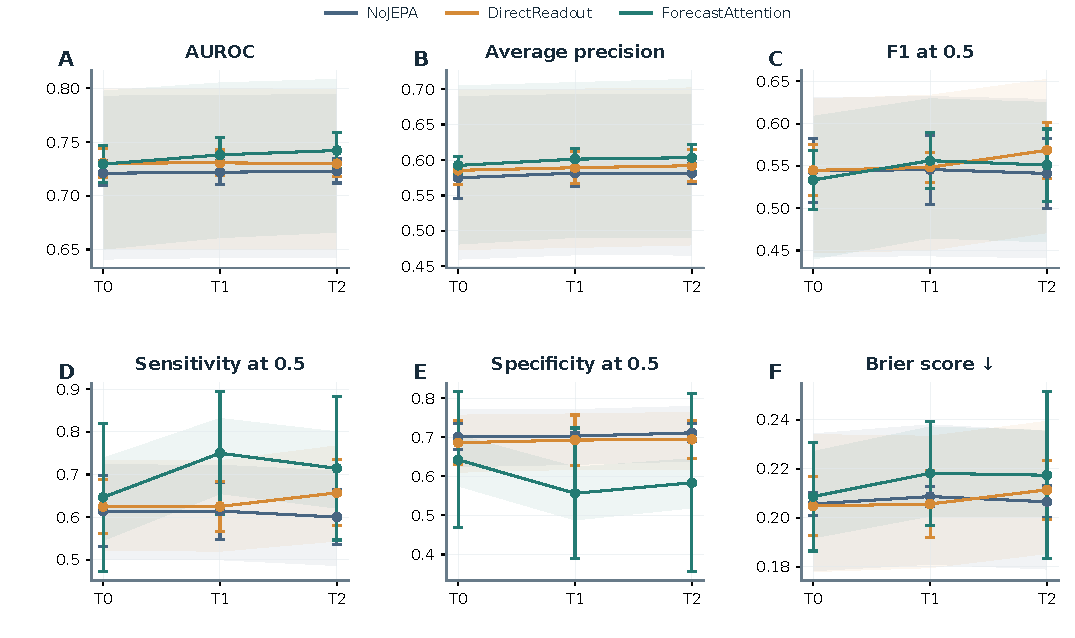
\includegraphics[width=\textwidth]{figures/landmark_performance.pdf}
\caption{Six complementary landmark summaries: AUROC, AP, F1, sensitivity, specificity, and Brier score. Metrics are computed separately for each seed-44 fold model and then equally averaged across five folds. Error bars show descriptive sample fold standard deviations, while shading gives conditional 95\% shared-patient-bootstrap intervals for the fold mean. All models and landmarks use the same 175 patients.}
\label{fig:longitudinal}
\end{figure*}

\begin{figure*}[t]
\centering
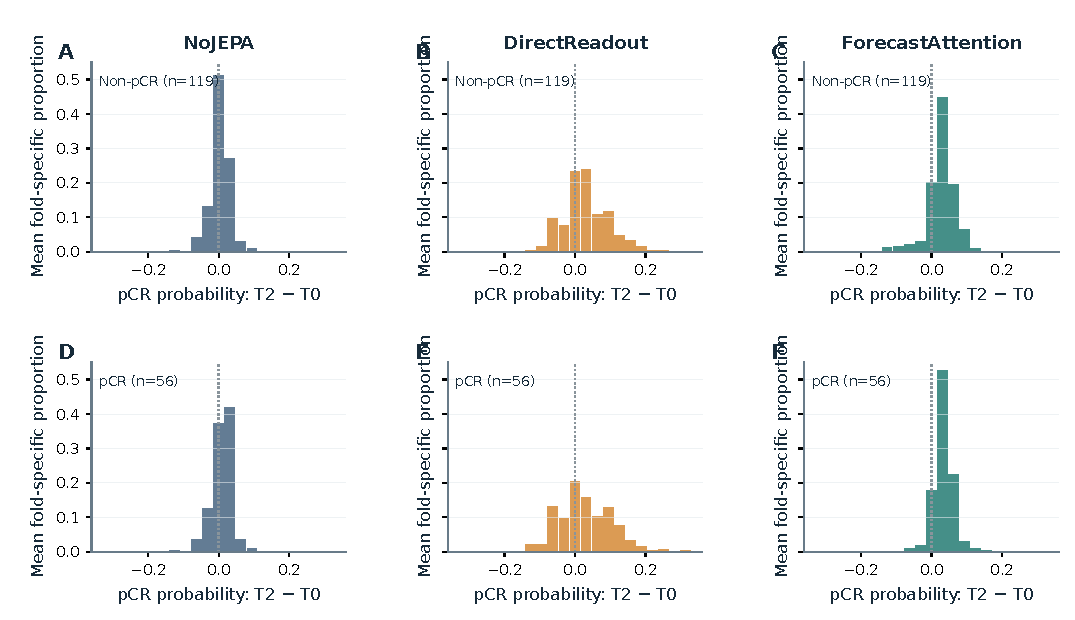
\includegraphics[width=\textwidth]{figures/outcome_score_changes.pdf}
\caption{Outcome-conditioned changes in predicted pCR probability from T0 to T2. Each fold model supplies one probability change per patient. Histograms are constructed separately within folds and then equally averaged; probabilities are not averaged between models. Panels separate variants and outcome classes. Repeated fold predictions are correlated observations of the same 175 patients and do not multiply the sample size by five. Score changes do not establish individual treatment effects.}
\label{fig:scorechanges}
\end{figure*}

\section{Supplementary subgroup and training-probe summaries}
\begin{table*}[t]
\centering
\small
\caption{Exploratory subgroup discrimination using seed 44, with each fold model evaluated separately. Model entries are means $\pm$ sample SD of five independently calculated fold metrics; Macro first averages T0--T2 within each fold. No prediction probabilities are averaged. Paired patient-bootstrap intervals for the mean ForecastAttention minus NoJEPA difference condition on the five fixed fold models. Age 50 is an exploratory reporting cutpoint. Namespace groups are parts of one clinical release, not external cohorts.}
\label{tab:subgroups}
\begin{tabular}{lrrr}
\toprule
Subgroup ($n$/pCR+) & NoJEPA & Full & $\Delta$ AUROC [95\% interval] \\
\midrule
HR+/HER2- (68/11) & 0.668 $\pm$ 0.032 & 0.701 $\pm$ 0.053 & +0.032 [-0.015, +0.081] \\
HR+/HER2+ (31/12) & 0.649 $\pm$ 0.022 & 0.607 $\pm$ 0.019 & -0.042 [-0.135, +0.046] \\
HR-/HER2+ (14/7) & 0.816 $\pm$ 0.075 & 0.824 $\pm$ 0.048 & +0.008 [-0.148, +0.148] \\
HR-/HER2- (62/26) & 0.637 $\pm$ 0.031 & 0.658 $\pm$ 0.033 & +0.022 [-0.024, +0.067] \\
Age $<$50 (90/29) & 0.667 $\pm$ 0.024 & 0.685 $\pm$ 0.028 & +0.017 [-0.008, +0.045] \\
Age $\geq$50 (85/27) & 0.781 $\pm$ 0.017 & 0.800 $\pm$ 0.009 & +0.018 [-0.018, +0.058] \\
ISPY2 namespace (125/39) & 0.679 $\pm$ 0.022 & 0.691 $\pm$ 0.011 & +0.012 [-0.016, +0.042] \\
ACRIN-6698 namespace (50/17) & 0.835 $\pm$ 0.026 & 0.857 $\pm$ 0.029 & +0.022 [-0.014, +0.063] \\
\bottomrule
\end{tabular}
\end{table*}

\begin{table*}[t]
\centering
\small
\caption{Archived seed44 epoch 20 fixed-training-probe diagnostics, shown as mean $\pm$ descriptive sample SD across five fold-specific statistics. Skill is $1-\mathrm{L1}_{forecast}/\mathrm{L1}_{copy}$ within each snapshot\textquotesingle s EMA coordinates; positive is better than holding the landmark state constant. Forecast targets require a continuous actually observed visit chain. These are training-probe summaries, not best-checkpoint holdout forecast evaluations. NoJEPA has no trained-world diagnostic.}
\label{tab:worldprobe}
\begin{tabular}{lrrr}
\toprule
Model & Horizon 1 skill & Horizon 2 skill & Horizon 3 skill \\
\midrule
NoJEPA & -- & -- & -- \\
DirectReadout & +0.026 $\pm$ 0.056 & +0.050 $\pm$ 0.142 & +0.193 $\pm$ 0.134 \\
ForecastAttention & -0.037 $\pm$ 0.016 & -0.015 $\pm$ 0.071 & +0.024 $\pm$ 0.028 \\
\bottomrule
\end{tabular}
\end{table*}


\section{Reproducibility and reporting items to complete}
The source package includes aggregate CSV files, source-report hashes, reproducible metric and figure scripts, the shared-patient-bootstrap procedure, and the official article class. The significance CSV includes raw $p$ values, within-family Holm adjustment, and adjustment over all 90 tests as a sensitivity analysis. It contains no patient identifiers, patient-level prediction rows, original MRI volumes, or model checkpoints. The method figure includes only rendered, anonymous development-image slices. Every variant uses training seed 44. Metrics are computed separately from each fold model's predictions before averaging across folds, with no probability ensembling. Archived training diagnostics are calculated in each model's own latent coordinates and summarized descriptively across folds.

\todo{Before submission, complete author and ethics statements; verify the precise pCR pathology definition; document codec and segmentation patient-level pretraining provenance; add matched external baselines and prospectively locked training and analysis policies; audit external-cohort independence; and confirm the journal's current submission and anonymization requirements.}
